\documentclass[14pt]{beamer}
\usetheme{Warsaw}
\usecolortheme{beaver}
\usefonttheme{professionalfonts}

\input{../../preamble}
\usepackage{amscd,amsmath,amssymb,amsthm,graphicx}
\usepackage[mathscr]{eucal}
\usepackage{paralist}
\usepackage{tabto}
\usepackage[normalem]{ulem}

% % % % % % % % % %
\title[Cal I S2015]{MATH 2554 (Calculus I)}
\subtitle{}
\author[Wheeler]{Dr. Ashley K. Wheeler}
\institute{University of Arkansas}
\date{\today}
\logo{}

% % %
\begin{document}
\maketitle

% % %
\begin{frame}
\frametitle{Table of Contents}
\tableofcontents
\end{frame}

% % %
\begin{frame}
\section[Week 1]{Week 1: 12-17 January}
\frametitle{Monday 12 January (Week 1)}
\begin{itemize}
\item Syllabus: go to 

{\footnotesize\url{comp.uark.edu/~ashleykw/Cal1S2015/cal1s15.html}}
\item MAA quiz tomorrow
\item Thurs 15 Jan Quiz 1 -- In general, quizzes are on Thursdays, take-home, and due Tuesdays.  When submitting a quiz, please:
	\begin{itemize}
	\item staple!
	\item defringe!
	\item write your name on every page!
	\item keep the questions in order!
	\end{itemize}
\item 1st WebHW is live.
\end{itemize}
\end{frame}

% % %
\begin{frame}
\frametitle{Tips for Success}
\small
\begin{itemize}
\item Attend class \& drills regularlly, pay attention, \uline{and participate}, take notes, and ask questions.
\item Complete HW on time and DON'T GET BEHIND!
\item Be sure to seek assistance (tutoring, office hours, etc.) if you are struggling.
\item Don't rely on success in high school calculus to save you in college calculus.
\item Find a study partner(s) to meet with on a regular basis to cover questions and study for quizzes/exams.
\item REMEMBER... THE SEMESTER STARTS TODAY!  SO DOES THE EVENTUAL EARNING OF YOUR FINAL GRADE!!!
\end{itemize}
\end{frame}

% % % 
\begin{frame}
\subsection[2.1 The Idea of Limits]{$\oint$ 2.1 The Idea of Limits}
\frametitle{$\oint$ 2.1 The Idea of Limits}
\begin{que} How would you define, and the differentiate between, the following pairs of terms? 
\begin{itemize}
\item instantaneous velocity vs. average velocity?
\item tangent line vs. secant line? 
\end{itemize}
\end{que}

(Recall:  What is a tangent line and what is a secant line?)
\end{frame}

% % %
\begin{frame}
\small
An object is launched into the air, and its position $s$ (in feet) at any time $t$ (in seconds) is given by the equation:
\[s(t)=-4.9t^2+30t+20.\]
\begin{itemize}
\item[1.] Compute the average velocity of the object over the following time intervals:  $[1,3],\,[1,2],\,[1,1.5]$
\item[2.] As your interval gets shorter, what do you notice about the average velocities?  What do you think would happen if we computed the average velocity of the object over the interval $[1,1.2]$? $[1,1.1]$? $[1,1.05]$?
\end{itemize}
\end{frame}

% % %
\begin{frame}
\begin{itemize}
\item[3.] How could you use the average velocities to estimate the instantaneous velocity at $t=1$?

\vspace{2pc}
\item[4.] What do the average velocities you computed in 1.\ represent on the graph of $s(t)$?
\end{itemize}
\end{frame}

% % %
\begin{frame}
\begin{que} What happens to the relationship between instantaneous velocity and average velocity as the time interval gets shorter? \end{que}

\vspace{2pc}
\pause 
The instantaneous velocity at $t=1$ is the limit of the average velocities as $t$ approaches 1.
\end{frame}

% % %
\begin{frame}
\begin{que} What is the relationship between the secant lines and the tangent lines as the time interval gets shorter? \end{que}

\vspace{2pc}
\pause
The slope of the tangent line at $(1, 45.1=s(1))$ is the limit of the slopes of the secant lines as $t$ approaches 1.
\end{frame}

% % %
\begin{frame}
\frametitle{HW from Section 2.1}
Do problems 1--3, 7, 9, 11, 13, 17, and 21.
\end{frame}

% % % % % % % % % % Wed 14 Jan 2015
\begin{frame}
\frametitle{Wednesday 14 January (Week 1)}
\footnotesize
\begin{itemize}
\item Syllabus: go to \url{comp.uark.edu/~ashleykw/Cal1S2015/cal1s15.html}
\item Thurs 15 Jan Quiz 1 -- In general, quizzes are on Thursdays, take-home, and due Tuesdays.  When submitting a quiz, please:
	\begin{itemize}\footnotesize
	\item staple!
	\item defringe!
	\item write your name on every page!
	\item keep the questions in order!
	\end{itemize}
\item 1st WebHW is live.  Follow the instructions on the syllabus for logging into MLP.
\item Recall: Opening activity from Monday.
\end{itemize}
\end{frame}

% % %
\begin{frame}
\subsection[2.2 Definition of Limits]{$\oint$ 2.2 Definition of Limits}
\frametitle{$\oint$ 2.2 Definition of Limits}
{\bf Determining Limits from a Graph:}
\begin{columns}[T]
\begin{column}{.5\textwidth}
\begin{block}
\centering{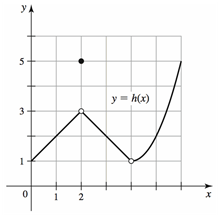
\includegraphics[scale=0.8]{Ch2Sect2_Exer7}}
\end{block}
\end{column}
\begin{column}{.5\textwidth}
\begin{block}
{Determine the following:}
\begin{itemize}
\item[1.] $h(1)$
\item[2.] $h(2)$
\item[3.] $h(4)$
\item[4.] $\displaystyle\lim_{x \to 2} h(x)$
\item[5.] $\displaystyle\lim_{x \to 4} h(x)$
\item[6.] $\displaystyle\lim_{x \to 1} h(x)$
\end{itemize}
\end{block}
\end{column}
\end{columns}
\end{frame}

% % %
\begin{frame}
\begin{que} Does $\displaystyle\lim_{x \to a} f(x)$ always equal $f(a)$? \end{que}
\end{frame}

% % %
\begin{frame}
\frametitle{}
{\bf Determining Limits from a Table:}

\vspace{1.5pc}
\small 
Suppose $f(x)=\dfrac{x^2+x-20}{x-4}.$

\vspace{1pc}
Create a table of values of $f(x)$ when
\begin{alignat*}{3}
x &= 3.9, 3.99, 3.999,\ \text{and}\\
x &= 4.1, 4.01, 4.001
\end{alignat*}
\begin{que}What can you conjecture about $\displaystyle\lim_{x \to 4} f(x)$? \end{que}
\end{frame}

% % %
\begin{frame}
\frametitle{Definitions of One-Sided Limits}
Notice in the previous example we can approach $f(x)$ from both sides as $x$ approaches $a$ (e.g., when $x>a$ and when $x<a$).  Up to this point we have been working with two-sided limits; however, for some functions it makes sense to examine one-sided limits.
\end{frame} 

% % %
\begin{frame}
\frametitle{}{\bf Right-hand limit:}  Suppose $f$ is defined for all $x$ near $a$ with $x>a$.  If $f(x)$ is arbitrarily close to $L$ for all $x$ sufficiently close to $a$ with $x>a$, we write
$$\lim_{x \to a^+} f(x)=L$$ 
and say the limit of $f(x)$ as $x$ approaches $a$ from the right equals $L$.
\end{frame}

% % %
\begin{frame}
\frametitle{}
{\bf Left-hand limit:}  Suppose $f$ is defined for all $x$ near $a$ with $x<a$.  If $f(x)$ is arbitrarily close to $L$ for all $x$ sufficiently close to $a$ with $x<a$, we write
$$\lim_{x \to a^-} f(x)=L$$ 
and say the limit of $f(x)$ as $x$ approaches $a$ from the left equals $L$.
\end{frame}

% % %
\begin{frame}
\frametitle{}
{\bf Determining One- and Two-Sided Limits:}
\begin{columns}[T]
\begin{column}{.5\textwidth}
\begin{block}
\centering{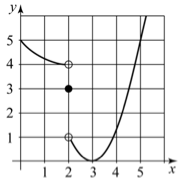
\includegraphics[scale=1.1]{Ch2Sect2_QQ7}}
\end{block}
\end{column}
\begin{column}{.5\textwidth}
\begin{block}
{Determine the following:}
\begin{itemize}
\item[1.] $g(2)$
\item[2.] $\displaystyle\lim_{x \to 2^+} g(x)$
\item[3.] $\displaystyle\lim_{x \to 2^-} g(x)$
\item[4.] $\displaystyle\lim_{x \to 2} g(x)$
\end{itemize}
\end{block}
\end{column}
\end{columns}
\end{frame}

% % %
\begin{frame}
\frametitle{\small Theorem Regarding Relationship Between One- and Two-Sided Limits}
\begin{thm}Assume $f$ is defined for all $x$ near $a$ except possibly at $a$.  Then 
\[\lim_{x \to a} f(x)=L\] if and only if 
\[\lim_{x \to a^+} f(x)=L\quad\text{ and }\quad\lim_{x \to a^-} f(x)=L.\]
\end{thm}
\end{frame}

\begin{frame}
\frametitle{HW from Section 2.2}
Do problems 1--4, 10, 12, 16, 18, 20, and 25 (pp.\ 61--63 in textbook)
\end{frame}

% % % % % % % % % % Fri 16 Jan 2015
\begin{frame}
\frametitle{Friday 16 January (Week 1)}
\small
\begin{itemize}
\item For old Calculus materials, see \url{comp.uark.edu/~ashleykw} and look for links under "Courses I've taught".  Last semester's in-class exam solutions are posted in there, too.
\item Thurs 23 Jan 23 Quiz \#2 (in drill).  Reminder on quizzes:
	\begin{itemize}\footnotesize
	\item staple!
	\item defringe!
	\item write your name on every page!
	\item keep the questions in order!
	\end{itemize}
\item Sunday Jan 26:  Computer HWs \#1  and \#2 Due
\end{itemize}
\end{frame}

% % %
\begin{frame}
\subsection[2.3 Techniques for Computing Limits]{$\oint$ 2.3 Techniques for Computing Limits}
\frametitle{$\oint$ 2.3 Techniques for Computing Limits}
This section provides various laws and techniques for determining limits.  These constitute {\bf analytical} methods of finding limits.  For example:

\vspace{1pc}
{\bf Limits of Linear Functions:}  Let $a$, $b$, and $m$ be real numbers.  For linear functions $f(x)=mx+b$,
\[\lim_{x \to a} f(x)=f(a)=ma+b.\]
\end{frame}

% % %
\begin{frame}
\frametitle{Limit Laws}
\small
Assume $\displaystyle\lim_{x \to a} f(x)$ and $\displaystyle\lim_{x \to a} g(x)$ exist.  

The following properties hold, where $c$ is a real number and $m$, $n$ are positive integers.

\vspace{0.75pc}
\begin{itemize}
\item[{\bf 1.}] {\bf Sum:} $\displaystyle\displaystyle\lim_{x \to a} [f(x)+g(x)] = \displaystyle\displaystyle\lim_{x \to a} f(x)+\displaystyle\displaystyle\lim_{x \to a} g(x)$

\vspace{0.5pc}
\item[{\bf 2.}] {\bf Difference:} $\displaystyle\lim_{x \to a} [f(x)-g(x)] = \displaystyle\lim_{x \to a} f(x)-\displaystyle\lim_{x \to a} g(x)$
\end{itemize}
\end{frame}

% % %
\begin{frame}
\small
\begin{itemize}
\item[{\bf 3.}] {\bf Constant Multiple:} $\displaystyle\lim_{x \to a} [cf(x)] = c \displaystyle\lim_{x \to a} [f(x)]$

\vspace{0.75pc}
\item[{\bf 4.}] {\bf Product:}  $\displaystyle\lim_{x \to a} [f(x)g(x)] = \left[\displaystyle\lim_{x \to a} f(x)\right] \left[\displaystyle\lim_{x \to a} g(x)\right]$
\end{itemize}
\end{frame}

% % %

\begin{frame}
\begin{itemize}
\item[{\bf 5.}] {\bf Quotient:}  $\displaystyle\lim_{x \to a} \left[ \frac{f(x)}{g(x)} \right] = \frac{\displaystyle\lim_{x \to a} f(x)}{\displaystyle\lim_{x \to a} g(x)}$

\vspace{1.2pc}
(provided $\displaystyle\lim_{x \to a} g(x) \ne 0$)
\end{itemize}

\vspace{1pc}
\alert{Note:} Don't ignore the parentheticals!
\end{frame}

% % %
\begin{frame}
\small
\begin{itemize}
\item[{\bf 6.}] {\bf Power:} $\displaystyle\lim_{x \to a} [f(x)]^n = \left[ \displaystyle\lim_{x \to a} f(x) \right]^n$

\vspace{0.75pc}
\item[{\bf 7.}] {\bf Fractional Power:} $\displaystyle\lim_{x \to a} [f(x)]^{n/m} = \left[ \displaystyle\lim_{x \to a} f(x) \right]^{n/m}$ 

\vspace{0.75pc}
(provided $f(x) \ge 0$ for $x$ near $a$ if $m$ is even and $n/m$ is reduced to lowest terms)
\end{itemize}
\end{frame}

% % %
\begin{frame}
\small
Laws \#1--6 hold for one-sided limits as well.  But Law \#7 must be modified:

\begin{itemize}
\item[{\bf 7.}] {\bf Fractional Power (one-sided limits):} 
	\begin{itemize}
	\item $\displaystyle\lim_{x \to a^{\alert{+}}} [f(x)]^{n/m} = \left[ \displaystyle\lim_{x \to a^{\alert{+}}} f(x) \right]^{n/m}$

	\vspace{0.25pc}
	(provided $f(x) \ge 0$ for $x$ near $a$ \alert{with $x>a$}, if $m$ is even and $n/m$ is reduced to lowest terms)
	
	\vspace{0.75pc}
	\item $\displaystyle\lim_{x \to a^{\alert{-}}} [f(x)]^{n/m} = \left[ \displaystyle\lim_{x \to a^{\alert{-}}} f(x) \right]^{n/m}$ 
	
	\vspace{0.25pc}
	(provided $f(x) \ge 0$ for $x$ near $a$ \alert{with $x<a$}, if $m$ is even and $n/m$ is reduced to lowest terms)
	\end{itemize}
\end{itemize}
\end{frame}

% % %
\begin{frame}
\frametitle{\large Limits of Polynomials and Rational Functions}
\small
Assume that $p(x)$ and $q(x)$ are polynomials and $a$ is a constant.
\begin{itemize}
\item {\bf Polynomial functions:}  $\displaystyle\lim_{x \to a} p(x) = p(a)$

\vspace{0.75pc}
\item {\bf Rational functions:}  $\displaystyle\lim_{x \to a} \frac{p(x)}{q(x)} = \frac{p(a)}{q(a)}$ 

\vspace{0.5pc}
(provided $q(a) \ne 0$)
\end{itemize}
\end{frame}

% % %
\begin{frame}
\frametitle{Exercises}
\footnotesize
Use the limit laws to evaluate the following limits.
\begin{itemize}
\item[1.\quad] $\displaystyle\lim_{x \to 1} \left[ \frac{4f(x)g(x)}{h(x)} \right]$,

\vspace{0.25pc}
given that $\displaystyle\lim_{x \to 1} f(x)=5$, $\displaystyle\lim_{x \to 1} g(x)=-2$, and $\displaystyle\lim_{x \to 1} h(x)=-4$.

\vspace{0.25pc}
\item[2.\quad] $\displaystyle\lim_{x \to 3} \frac{4x^2+3x-6}{2x-3}$

\vspace{0.75pc}
\item[3.\quad] $\displaystyle\lim_{x \to 1^-}g(x)$ \;and\; $\displaystyle\lim_{x \to 1^+}g(x)$, 

\vspace{0.25pc}
given that 
$g(x) = 
\begin{cases}
x^2 & \text{if $x \le 1$}; \\
x+2 & \text{if $x>1$}.
\end{cases}$ 
\end{itemize}
\end{frame}

% % %
\begin{frame}
\frametitle{Additional (Algebra) Techniques}
\small
When direct substitution fails:

\vspace{0.5pc}
\begin{itemize}
\item[1.\quad] $\displaystyle\lim_{t \to 2} \frac{3t^2-7t+2}{2-t}$

\vspace{0.25pc}
{\footnotesize One strategy is to factor and see if the denominator can be cancelled out.}

\vspace{0.5pc}
\item[2.\quad] $\displaystyle\lim_{h \to 0} \frac{\displaystyle \frac{1}{5+h}-\frac{1}{5} }{h}$

\vspace{0.25pc}
{\footnotesize In general, review your algebra techniques, since they can save you some headache.}
\end{itemize}
\end{frame}

% % %

\begin{frame}
\frametitle{Another Technique: Squeeze Theorem}
\small
A final method for evaluating limits involves the relationship of functions with each other.
\footnotesize
\begin{thm}[Squeeze Theorem]  Assume the functions $f$, $g$, and $h$ are functions and 
\[f(x)\le g(x) \le h(x)\] 
for all values of $x$ near $a$, except possibly at $a$.  If 
\[\displaystyle\lim_{x \to a}f(x)=\displaystyle\lim_{x \to a} h(x)=L,\] 
then 
\[\displaystyle\lim_{x \to a} g(x)=L.\] \end{thm}
\end{frame}

% % %
\begin{frame}
Example: 

\vspace{0.5pc}
\begin{itemize}
\item[(a)]Draw a graph of the inequality 
\[-|x| \le x^2 \ln x^2 \le |x|.\]

\vspace{0.5pc}
\item[(b)] Compute $\displaystyle\lim_{x \to 0} x^2 \ln x^2.$
\end{itemize}
\end{frame}

% % %
\begin{frame}
\frametitle{HW from Section 2.3}
Do problems 12--30 (every 3rd problem), 31, 33, 37--47 odds, 51, 53, 61--65 odds (pp.\ 73--75 in textbook).
\end{frame}

\begin{comment}
\end{comment}

\end{document}